%%%%%%%%%%%%%%%%%%%%%%%%%%%%%%%%%%%%%%%%%%%%%%%%%%%%%%%%%%%%%%%%%%%%%%%%%%%%%%%
%%  Snake Game OS -- IEEE Conference Report
%%  Author: Madhav
%%  Compiles on Overleaf with the default pdfLaTeX engine.
%%%%%%%%%%%%%%%%%%%%%%%%%%%%%%%%%%%%%%%%%%%%%%%%%%%%%%%%%%%%%%%%%%%%%%%%%%%%%%%

\documentclass[conference]{IEEEtran}
\IEEEoverridecommandlockouts

\usepackage{cite}
\usepackage{amsmath,amssymb,amsfonts}
\usepackage{algorithmic}
\usepackage{graphicx}
\usepackage{textcomp}
\usepackage{xcolor}
\usepackage{listings}
\usepackage{url}
\usepackage{hyperref}
\usepackage[section]{placeins}  % keeps figures inside their section
\usepackage{float}              % provides the [H] specifier
\usepackage{tikz}
\usetikzlibrary{positioning,arrows.meta,shapes.geometric,fit,backgrounds,calc}

\hypersetup{
    colorlinks=true,
    linkcolor=black,
    citecolor=black,
    urlcolor=blue
}

% Code listing style for C
\lstdefinestyle{cstyle}{
    language=C,
    basicstyle=\ttfamily\scriptsize,
    keywordstyle=\color{blue!70!black}\bfseries,
    commentstyle=\color{green!50!black}\itshape,
    stringstyle=\color{red!70!black},
    numbers=left,
    numberstyle=\tiny\color{gray},
    stepnumber=1,
    numbersep=6pt,
    frame=single,
    rulecolor=\color{black!30},
    breaklines=true,
    captionpos=b,
    tabsize=2,
    showstringspaces=false
}
\lstset{style=cstyle}

\def\BibTeX{{\rm B\kern-.05em{\sc i\kern-.025em b}\kern-.08em
    T\kern-.1667em\lower.7ex\hbox{E}\kern-.125emX}}

\begin{document}

\title{Snake Game OS: A Real-Time Terminal Game\\
       Built on Custom System Libraries in C%
       \thanks{Source code and version history:
        \url{https://github.com/HackHeroic/Snake_game_os}}}

\author{
    \IEEEauthorblockN{C Murali Madhav}
    \IEEEauthorblockA{
        Roll No.\ 230115\\
        Newton School of Technology\\
        Rishihood University
    }
    \hspace{2em}
    \IEEEauthorblockN{Ravi Yadav}
    \IEEEauthorblockA{
        Roll No.\ 230131\\
        Newton School of Technology\\
        Rishihood University
    }
}

\maketitle

%==============================================================================
\begin{abstract}
This paper presents the design and implementation of \textit{Snake Game OS}, a real-time terminal-based Snake game written entirely in C using only \texttt{<stdio.h>} and \texttt{<stdlib.h>} from the C standard library. All other system-level facilities---string manipulation, arithmetic, dynamic memory allocation, screen rendering, and keyboard input---are implemented from first principles to demonstrate core operating systems concepts in a single self-contained application. The project incorporates the five canonical OS sub-systems: (i)~a custom \textbf{memory manager} that allocates a 64\,KB virtual RAM region at start-up and serves all subsequent requests through a first-fit allocator with block splitting and forward coalescing; (ii)~a cooperative \textbf{process/loop manager} structured as a deterministic real-time game loop with a three-state finite-state automaton (\textsc{Running}, \textsc{Paused}, \textsc{GameOver}); (iii)~an \textbf{I/O subsystem} that puts the terminal into raw mode through \texttt{termios}, reads non-blocking single-byte input, decodes multi-byte ANSI escape sequences for arrow keys, and renders frames using ANSI 256-colour escape codes with a delta-redraw strategy; (iv)~a lightweight \textbf{file system} layer that persists high scores and lifetime statistics to flat files using a fail-safe write strategy; and (v)~\textbf{security and halt-handling} mechanisms that capture SIGINT, restore terminal state on every exit path, validate dynamic memory bounds, reject illegal direction transitions, and bound spawn-loop iterations to guarantee progress. Optimal algorithmic choices (Russian-peasant multiplication, binary long-division, Schrage's overflow-safe MINSTD PRNG, linked-list snake body, delta rendering) are made in each module to maximise efficiency on commodity hardware. A separate \emph{Phase~2} branch extends the core engine with multi-food spawning, an autonomous ghost snake, animated power-up zones, a shrinking play area, persistent best-run replay, and dynamic terminal-resize handling. The system has been tested on macOS Darwin~25.4.0 with 65 passing unit tests across the math, string, and memory libraries, and the version history is maintained on a public GitHub repository.
\end{abstract}

\begin{IEEEkeywords}
operating systems, memory management, custom allocator, file system, process management, I/O management, terminal raw mode, ANSI escape codes, real-time game loop, C programming
\end{IEEEkeywords}

%==============================================================================
\section{Introduction}
\label{sec:intro}

Modern operating systems abstract five core resources for application programmers: \textit{processes}, \textit{memory}, \textit{files}, \textit{devices}, and \textit{security}~\cite{silberschatz2018,tanenbaum2014}. While these abstractions are usually hidden behind kernel APIs and standard library calls such as \texttt{malloc}, \texttt{printf}, and \texttt{strlen}, building a non-trivial application without these abstractions is highly instructive: it forces the engineer to confront the same trade-offs that real kernels resolve.

This work pursues exactly that pedagogical goal. \textit{Snake Game OS} is a real-time terminal Snake clone in which every system-level facility is hand-written in approximately 1{,}500 lines of C. The only standard headers permitted in the build are \texttt{<stdio.h>} and \texttt{<stdlib.h>}; \texttt{<string.h>}, \texttt{<math.h>}, and the standard \texttt{malloc}/\texttt{free} are forbidden inside the game logic. A single \texttt{malloc} call at start-up reserves a 64\,KB region that thereafter behaves as a virtual RAM managed entirely by user-space code.

The contributions of the report are:
\begin{enumerate}
    \item A complete, working implementation of the five OS sub-systems within a single, self-contained binary.
    \item Justified, optimal algorithmic choices in each module, e.g. $O(\log n)$ shift-and-add multiplication and binary long-division, an overflow-safe Schrage MINSTD PRNG~\cite{park1988}, a first-fit allocator with coalescing~\cite{knuth1997}, and a delta-render frame strategy for flicker-free output.
    \item A robust security/halt model in which every exit path---normal exit, user quit (\texttt{q}), \texttt{SIGINT} from the terminal, or fatal collision---restores the terminal to canonical mode and persists user data.
    \item A clean separation of concerns into three layers (\texttt{lib/}, \texttt{game/}, \texttt{ui/}) with a publicly maintained version history on GitHub.
    \item An advanced Phase~2 branch demonstrating multi-food, an autonomous ghost AI, power-up zones, a shrinking board, deterministic-replay ghosts, and \texttt{SIGWINCH}-aware resize recovery (Section~\ref{sec:phase2}).
    \item A reproducible, scripted screenshot pipeline that drives the binary via \texttt{tmux} and renders every game state to PNG without manual capture (Section~\ref{sec:results}).
\end{enumerate}

The remainder of the paper is organised as follows. Section~\ref{sec:related} surveys related work. Section~\ref{sec:arch} introduces the overall architecture. Section~\ref{sec:methodology} (Methodology) describes each OS sub-system in detail. Section~\ref{sec:results} reports build and test results. Section~\ref{sec:future} discusses future scope and Section~\ref{sec:conclusion} concludes.

%==============================================================================
\section{Related Work}
\label{sec:related}

Terminal-based games have a long history as teaching vehicles for low-level systems programming. The original UNIX \texttt{rogue} (1980) popularised \texttt{curses}-based rendering, and the GNU \texttt{ncurses} library remains the de-facto choice for portable terminal interfaces today~\cite{ncurses}. The present work deliberately avoids \texttt{ncurses} and re-implements a minimal subset of its functionality directly atop \texttt{termios} and ANSI escape codes, in order to expose the underlying mechanism rather than hide it.

Custom memory allocators have been studied extensively since Knuth's analysis of fit policies in \textit{The Art of Computer Programming}~\cite{knuth1997}. Wilson \emph{et al.}~\cite{wilson1995} provide a comprehensive survey of dynamic storage allocation; the simple first-fit-with-coalescing scheme used here is one of the oldest documented designs and is sufficient for the modest memory footprint of a Snake game.

Pseudo-random number generation in fixed-size integer arithmetic was treated by Park and Miller~\cite{park1988}, who recommended the multiplicative congruential generator $X_{n+1} = 16807 \, X_n \bmod (2^{31}-1)$. Schrage~\cite{schrage1979} showed how to implement this generator in 32-bit integers without overflow. We adopt this exact construction.

%==============================================================================
\section{System Architecture}
\label{sec:arch}

Figure~\ref{fig:architecture} shows the three-layer architecture. Each layer depends only on the layers below it.

\begin{figure}[H]
    \centering
    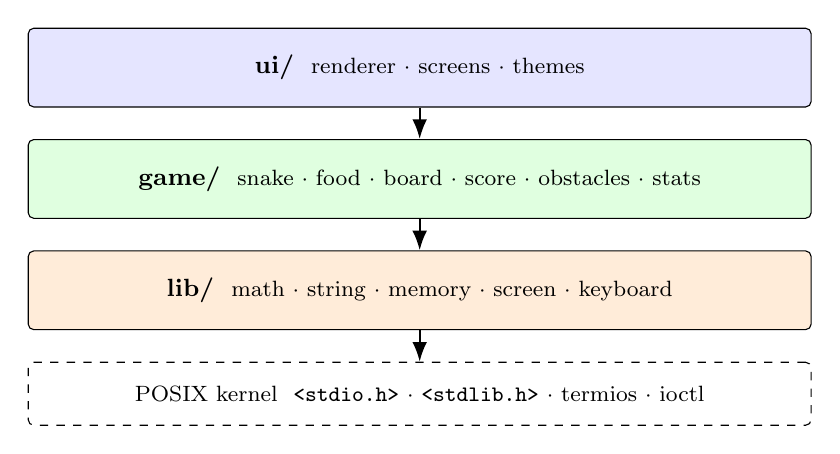
\begin{tikzpicture}[
        layer/.style={
            draw, rounded corners=2pt, minimum width=0.82\columnwidth,
            minimum height=10mm, align=center, font=\small
        },
        ui/.style={layer, fill=blue!10},
        gm/.style={layer, fill=green!12},
        lb/.style={layer, fill=orange!15},
        flow/.style={-{Latex[length=2.5mm]}, thick}
    ]
        \node[ui] (ui) {\textbf{ui/} \ \footnotesize renderer\ $\cdot$\ screens\ $\cdot$\ themes};
        \node[gm, below=4mm of ui] (game)
            {\textbf{game/} \ \footnotesize snake\ $\cdot$\ food\ $\cdot$\ board\ $\cdot$\ score\ $\cdot$\ obstacles\ $\cdot$\ stats};
        \node[lb, below=4mm of game] (lib)
            {\textbf{lib/} \ \footnotesize math\ $\cdot$\ string\ $\cdot$\ memory\ $\cdot$\ screen\ $\cdot$\ keyboard};
        \node[draw, dashed, rounded corners=2pt, minimum width=0.82\columnwidth,
              minimum height=8mm, below=4mm of lib, align=center, font=\footnotesize]
              (os) {POSIX kernel\ \ \texttt{<stdio.h>}\ $\cdot$\ \texttt{<stdlib.h>}\ $\cdot$\ termios\ $\cdot$\ ioctl};
        \draw[flow] (ui) -- (game);
        \draw[flow] (game) -- (lib);
        \draw[flow] (lib) -- (os);
    \end{tikzpicture}
    \caption{Three-layer architecture: UI depends on game logic, game logic depends on system libraries, system libraries depend only on \texttt{<stdio.h>}, \texttt{<stdlib.h>}, and POSIX headers.}
    \label{fig:architecture}
\end{figure}

\begin{itemize}
    \item \textbf{\texttt{lib/}} contains the system-level libraries: \texttt{math.c}, \texttt{string.c}, \texttt{memory.c}, \texttt{screen.c}, \texttt{keyboard.c}. They have zero knowledge of the game.
    \item \textbf{\texttt{game/}} contains pure game logic: \texttt{snake.c}, \texttt{food.c}, \texttt{board.c}, \texttt{score.c}, \texttt{obstacles.c}, \texttt{stats.c}. These modules manipulate state but never draw.
    \item \textbf{\texttt{ui/}} contains all rendering: \texttt{renderer.c}, \texttt{screens.c}, \texttt{themes.c}. It reads game state and emits ANSI sequences via \texttt{lib/screen.c}.
    \item \textbf{\texttt{main.c}} orchestrates the lifecycle: initialisation, the game loop, and shutdown.
\end{itemize}

This separation enforces two valuable invariants: (1) the game module is fully testable without a terminal, and (2) replacing the rendering back-end (e.g.\ swapping ANSI for SDL) requires touching only \texttt{ui/}.

%==============================================================================
\section{Methodology}
\label{sec:methodology}

This section describes the design and rationale of each operating-systems sub-system. The five sub-systems on the project's evaluation rubric --- memory management, process management, I/O management, file systems, and security/halt-handling --- are presented in the order in which they are exercised at run time, from the lowest-level abstraction up.

%------------------------------------------------------------------------------
\subsection{Memory Management}
\label{sec:mem}

\subsubsection{Design}
At program start, \texttt{memory\_init()} performs the \emph{only} call to the standard \texttt{malloc} in the entire game logic, requesting a single 64\,KB block (\texttt{VIRTUAL\_RAM\_SIZE = 65536}). All subsequent allocations and de-allocations are served by a custom first-fit allocator that operates inside this block. Conceptually, this is the user-space analogue of a kernel's heap manager.

\subsubsection{Block Layout}
Each block is preceded by an 8-byte aligned header:
\begin{equation*}
\underbrace{[\text{size: 4B}]}_{\text{user-data size}} \;
\underbrace{[\text{in\_use: 1B}]}_{\text{0=free, 1=alloc}} \;
\underbrace{[\text{padding: 3B}]}_{\text{align to 8B}} \;
\underbrace{[\text{user data \dots}]}_{\text{returned to caller}}
\end{equation*}
The 3-byte padding ensures the user pointer is 8-byte aligned, which is sufficient on the target architectures (x86-64 and ARM64).

\subsubsection{Allocation Algorithm}
\texttt{alloc(size)} performs first-fit traversal of the block list (Listing~\ref{lst:alloc}). On finding a sufficient free block, it splits the block only if the remainder can hold a header plus the minimum 8-byte payload (\texttt{MIN\_SPLIT = 16}). This avoids creating un-usable splinters.

\begin{lstlisting}[caption={First-fit allocator with conditional splitting (excerpt from \texttt{src/lib/memory.c}).},label={lst:alloc}]
ptr = virtual_ram;
while (ptr < virtual_ram + VIRTUAL_RAM_SIZE) {
    block = (BlockHeader *)ptr;
    if (!block->in_use && block->size >= size) {
        if (block->size >= size + MIN_SPLIT) {
            BlockHeader *next = (BlockHeader *)
                (ptr + HEADER_SIZE + size);
            next->size = block->size - size - HEADER_SIZE;
            next->in_use = 0;
            block->size = size;
        }
        block->in_use = 1;
        return ptr + HEADER_SIZE;
    }
    ptr += HEADER_SIZE + block->size;
}
return NULL;
\end{lstlisting}

\subsubsection{Forward Coalescing}
\texttt{dealloc()} marks a block free and then walks forward, merging contiguous free blocks into one (Listing~\ref{lst:dealloc}). Figure~\ref{fig:mem} shows the heap after several allocations and one free, with adjacent free regions coalesced. Forward-only coalescing is sufficient because every allocation traverses from the start of the heap, so two adjacent free blocks are guaranteed to be merged on the next allocation that targets the earlier of the two. This avoids the bookkeeping of doubly-linked free lists while still preventing unbounded fragmentation.

\begin{lstlisting}[caption={Constant-time deallocation followed by greedy forward coalescing.},label={lst:dealloc}]
block = (BlockHeader *)((char *)user_ptr - HEADER_SIZE);
block->in_use = 0;

/* forward coalescing: absorb every contiguous free neighbour */
ptr = (char *)block + HEADER_SIZE + block->size;
while (ptr < virtual_ram + VIRTUAL_RAM_SIZE) {
    next = (BlockHeader *)ptr;
    if (next->in_use) break;
    block->size += HEADER_SIZE + next->size;
    ptr += HEADER_SIZE + next->size;
}
\end{lstlisting}

\subsubsection{Why First-Fit?}
The Snake game's working set is small (a few hundred bytes for the snake linked list, plus a handful of game-object structs), and allocations are highly homogeneous in size. Under such workloads, first-fit with coalescing has been shown by Wilson \emph{et al.}~\cite{wilson1995} to perform comparably to best-fit while being substantially simpler and faster. Best-fit was rejected because it offers no measurable benefit at this scale and would cost a full traversal even on hits.

\subsubsection{Memory-Pressure Handling}
\texttt{alloc()} returns \texttt{NULL} on exhaustion. All callers that allocate (\texttt{snake\_create}, \texttt{snake\_move}, \texttt{food\_spawn}, \texttt{board\_create}, \texttt{score\_create}) explicitly check the return value and degrade gracefully: a failed move simply skips the tick, a failed spawn returns \texttt{NULL} and the caller treats the board as full (triggering victory).

\begin{figure}[H]
    \centering
    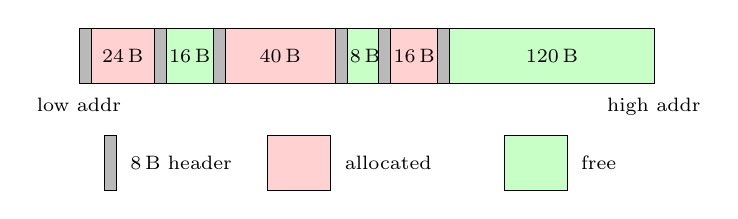
\begin{tikzpicture}[
        x=1mm, y=1mm,
        block/.style={draw, minimum height=7mm, font=\scriptsize, align=center, inner sep=1pt},
        used/.style ={block, fill=red!18},
        free/.style ={block, fill=green!22},
        hdr/.style  ={draw, fill=gray!55, minimum width=1.5mm, minimum height=7mm, inner sep=0pt}
    ]
        % heap strip: header tick + body block, 6 blocks total ~80mm wide
        \def\bx{0}
        \foreach \kind/\sz/\lbl in {%
            used/8/24, free/6/16, used/14/40, free/4/8, used/6/16, free/26/120%
        }{
            \pgfmathsetmacro{\bodyx}{\bx + 1.5}
            \node[hdr,  anchor=south west] at (\bx, 0) {};
            \node[\kind, anchor=south west, minimum width=\sz mm]
                  at (\bodyx, 0) {\lbl\,B};
            \pgfmathsetmacro{\nbx}{\bodyx + \sz}
            \xdef\bx{\nbx}
        }
        % low/high address labels under the strip
        \node[font=\scriptsize, anchor=north] at (0, -0.5)   {low addr};
        \node[font=\scriptsize, anchor=north] at (\bx, -0.5) {high addr};
        % legend (well below the strip)
        \node[hdr,  label=right:{\scriptsize\,8\,B header}] at (4,  -10) {};
        \node[used, minimum width=8mm,
              label=right:{\scriptsize\,allocated}]         at (28, -10) {};
        \node[free, minimum width=8mm,
              label=right:{\scriptsize\,free}]              at (58, -10) {};
    \end{tikzpicture}
    \caption{Logical layout of the 64\,KB virtual RAM after several allocations and one free. Each block is preceded by an 8-byte header (\textsc{H}); adjacent free regions are coalesced lazily on the next \texttt{dealloc}.}
    \label{fig:mem}
\end{figure}

%------------------------------------------------------------------------------
\subsection{Process Management}
\label{sec:proc}

Although the game is single-threaded, the design is informed by classical process-management ideas: a finite-state machine, deterministic scheduling, and well-defined transitions.

\subsubsection{Real-Time Game Loop}
The body of \texttt{main()} (Listing~\ref{lst:loop}) is structured as a deterministic loop where each iteration corresponds to one game tick. The tick period is data-driven: \texttt{score\_get\_speed()} returns a delay $d$ (in milliseconds) computed as
\begin{equation}
d = \max\left(80,\; 200 - 15 \cdot \mathrm{level}\right)
\end{equation}
and the loop sleeps for $d \cdot 1000$ microseconds via \texttt{usleep}. This is a cooperative one-shot scheduler with a single ready task; there is no preemption.

\begin{lstlisting}[caption={Skeleton of the game-loop scheduler.},label={lst:loop}]
while (snake->alive) {
    key = read_key();          /* non-blocking */
    handle_quit_pause(key);
    update_direction(key);
    compute_next_head(...);
    check_wall_or_wrap(...);
    check_self_collision(...);
    check_obstacle_collision(...);
    move_snake(...);
    update_score_and_spawn_food(...);
    render_delta(...);
    usleep(score_get_speed(score) * 1000);
}
\end{lstlisting}

\subsubsection{Finite-State Automaton}
The game has three logical states---\textsc{Running}, \textsc{Paused}, and \textsc{GameOver}---with transitions driven by key presses (\texttt{P}, \texttt{Q}) and lethal events. Figure~\ref{fig:fsm} depicts the FSM.

\begin{figure}[H]
    \centering
    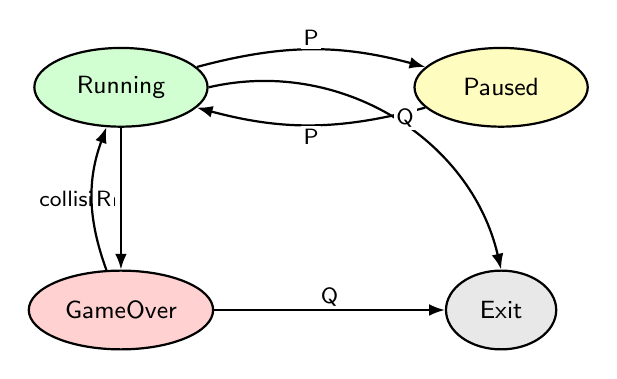
\begin{tikzpicture}[
        node distance=18mm and 26mm,
        state/.style={
            ellipse, draw, thick, minimum width=22mm, minimum height=10mm,
            font=\small\sffamily, align=center
        },
        run/.style ={state, fill=green!18},
        pa/.style  ={state, fill=yellow!25},
        go/.style  ={state, fill=red!18},
        ex/.style  ={state, fill=gray!18, minimum width=14mm},
        arrow/.style ={->, thick, >={Latex[length=2mm]}},
        lab/.style ={font=\footnotesize\sffamily, fill=white, inner sep=1pt}
    ]
        \node[run] (R)                 {Running};
        \node[pa,  right=of R] (P)     {Paused};
        \node[go,  below=of R] (G)     {GameOver};
        \node[ex,  below=of P] (E)     {Exit};

        \draw[arrow] (R) to[bend left=15]  node[lab, above]{P}         (P);
        \draw[arrow] (P) to[bend left=15]  node[lab, below]{P}         (R);
        \draw[arrow] (R) to                node[lab, left] {collision} (G);
        \draw[arrow] (G) to[bend left=20]  node[lab, right]{R}         (R);
        \draw[arrow] (G) to                node[lab, above]{Q}         (E);
        \draw[arrow] (R.east) to[bend left=45] node[lab, right]{Q}     (E.north);
    \end{tikzpicture}
    \caption{Finite-state automaton governing the game lifecycle. \texttt{P} toggles pause; a wall, self, or obstacle collision drives \textsc{Running} into \textsc{GameOver}; \texttt{R} restarts; \texttt{Q} exits from any state.}
    \label{fig:fsm}
\end{figure}

\subsubsection{Pause Semantics}
While \textsc{Paused}, the loop sleeps $50$\,ms per iteration and only polls the keyboard, consuming negligible CPU. This mirrors how a real OS suspends a process: it remains in a known state but performs no user work. On unpause, the screen is fully redrawn to recover from any terminal scrollback that may have occurred.

\subsubsection{Determinism and Reproducibility}
The pseudo-random seed is initialised from the time elapsed (in iterations) on the title screen, but once the game starts the entire trajectory is a pure function of the seed and the input sequence. This is the same property that simplifies debugging in real OS schedulers using deterministic replay~\cite{tanenbaum2014}.

%------------------------------------------------------------------------------
\subsection{I/O Management}
\label{sec:io}

The I/O subsystem is split into two complementary modules: \texttt{lib/keyboard.c} for input and \texttt{lib/screen.c} (driven by \texttt{ui/renderer.c}) for output.

\subsubsection{Raw Mode Keyboard}
By default, terminals operate in \emph{cooked} (canonical) mode, buffering input until a newline is received and echoing characters back to the screen. Real-time games require \emph{raw} mode. The function \texttt{keyboard\_init()} (Listing~\ref{lst:raw}) clears the \texttt{ECHO}, \texttt{ICANON}, and \texttt{ISIG} flags via \texttt{termios}~\cite{posix}, and sets \texttt{VMIN=0, VTIME=0} for fully non-blocking reads. The original termios are saved and restored on every exit path.

\begin{lstlisting}[caption={Switching the terminal into raw, non-blocking mode.},label={lst:raw}]
tcgetattr(STDIN_FILENO, &original_termios);
raw = original_termios;
raw.c_lflag &= ~(ECHO | ICANON | ISIG);
raw.c_cc[VMIN]  = 0;
raw.c_cc[VTIME] = 0;
tcsetattr(STDIN_FILENO, TCSAFLUSH, &raw);
signal(SIGINT, sigint_handler);
\end{lstlisting}

\subsubsection{Arrow-Key Decoding}
Arrow keys arrive as the three-byte sequence \texttt{ESC \texttt{[} A/B/C/D}. \texttt{read\_key()} consumes the lead-in \texttt{0x1B} and reads the next two bytes to disambiguate. WASD letters share the same logical mapping for ergonomic redundancy.

\subsubsection{Three-Byte Escape Decoder}
The lead-in byte for an arrow key is \texttt{0x1B}, which on its own may simply mean ``the user pressed Escape''. The decoder (Listing~\ref{lst:keydecode}) reads two further bytes; if they form the prefix \texttt{[A/B/C/D} the key is mapped to a logical \texttt{KEY\_UP/DOWN/RIGHT/LEFT} constant, otherwise the lone \texttt{ESC} is returned. Because the second and third \texttt{read()} calls are also non-blocking they cannot deadlock when the user genuinely typed only \texttt{ESC}.

\begin{lstlisting}[caption={Non-blocking ANSI arrow-key decoder.},label={lst:keydecode}]
if (c == '\033') {
    unsigned char seq[2];
    if (read(STDIN_FILENO, &seq[0], 1) != 1) return '\033';
    if (read(STDIN_FILENO, &seq[1], 1) != 1) return '\033';
    if (seq[0] == '[') {
        switch (seq[1]) {
            case 'A': return KEY_UP;
            case 'B': return KEY_DOWN;
            case 'C': return KEY_RIGHT;
            case 'D': return KEY_LEFT;
        }
    }
    return '\033';
}
\end{lstlisting}

\subsubsection{Output via ANSI Escape Codes}
\texttt{lib/screen.c} wraps the small set of ANSI escape sequences~\cite{ansi} needed by the game:
\begin{itemize}
    \item Cursor positioning: \texttt{\textbackslash 033[y;xH}
    \item 256-colour foreground: \texttt{\textbackslash 033[38;5;Nm}
    \item Cursor hide/show: \texttt{\textbackslash 033[?25l} / \texttt{\textbackslash 033[?25h}
    \item Clear screen: \texttt{\textbackslash 033[2J\textbackslash 033[H}
\end{itemize}

\subsubsection{Delta Rendering}
A naive renderer that clears and redraws the entire frame every tick would flicker visibly even at 200\,ms per tick. Instead, the renderer uses a \textit{delta} strategy: only the changed cells are emitted to \texttt{stdout}. Concretely, on each tick the renderer (i)~erases the cell vacated by the tail (unless the snake grew), (ii)~draws the new head, and (iii)~updates the HUD only when the score has changed. Borders, obstacles, and food are emitted exactly once on spawn. The cursor is hidden during play, eliminating visual chatter.

This optimisation reduces the per-tick character count from roughly $W \cdot H$ (full frame) to fewer than ten bytes, well under any conceivable terminal bandwidth bottleneck. Listing~\ref{lst:delta} shows the post-move render block at the heart of this strategy: only the vacated tail cell is erased, only the head is painted, and the HUD is touched solely when the score has actually changed.

\begin{lstlisting}[caption={Delta-render hot path: O(1) per tick, regardless of snake length.},label={lst:delta}]
if (grew) {
    /* food was eaten -- snake grows, no tail erase needed */
    food_free(food);
    food = food_spawn(snake, &obstacles, board_w, board_h, &seed);
    if (food) render_food(food, board, theme);
} else {
    /* normal move -- erase the cell the tail just vacated */
    render_erase_tail(old_tail_x, old_tail_y, board);
}
render_snake(snake, theme);                  /* repaints head only */
if (score->score != last_score) {            /* HUD: only when stale */
    render_hud(score, board);
    last_score = score->score;
}
screen_flush();
\end{lstlisting}

\subsubsection{Adaptive Board Sizing and Wrap-Around}
On start, \texttt{board.c} queries the current terminal dimensions via the \texttt{ioctl(\dots,\,TIOCGWINSZ,\dots)} call and computes a board sized to fill the terminal minus borders, margins, and HUD lines. A minimum size of $22 \times 14$ is enforced; otherwise the program halts with a clear error message. In Wrap-Around mode the head's coordinates are wrapped through a single modulo expression (Listing~\ref{lst:wrap}); the leading addition of \texttt{width}/\texttt{height} guarantees a non-negative argument so that the custom \texttt{my\_mod} returns the mathematically correct residue for both positive and negative inputs.

\begin{lstlisting}[caption={Branch-free toroidal wrap using the custom \texttt{my\_mod}.},label={lst:wrap}]
void board_wrap_position(Board *b, int *x, int *y) {
    *x = my_mod(*x + b->width,  b->width);
    *y = my_mod(*y + b->height, b->height);
}
\end{lstlisting}

%------------------------------------------------------------------------------
\subsection{File System}
\label{sec:fs}

The game persists two kinds of state to the local file system, illustrating two file-system patterns: a single-value file (high score) and a record file (lifetime stats).

\subsubsection{High-Score File}
The file \texttt{data/highscore.dat} holds a single ASCII integer. Functions \texttt{score\_save\_high()} and \texttt{score\_load\_high()} use \texttt{fopen}/\texttt{fprintf}/\texttt{fscanf} from \texttt{<stdio.h>}, with defensive defaults: if the file is absent on the first run, \texttt{score\_load\_high()} returns 0 silently rather than failing.

\subsubsection{Lifetime Statistics File}
The file \texttt{data/stats.dat} stores four space-separated integers: \texttt{games\_played}, \texttt{total\_food}, \texttt{longest\_snake}, \texttt{best\_level}. The format is intentionally human-readable so users can inspect or back up their data.

\subsubsection{Persistence Strategy}
Both files are loaded once at start-up. The lifetime statistics file is rewritten at every game-over \emph{and} on quit (\texttt{Q}) so progress survives even an abandoned run; the high-score file is rewritten only at game-over, since the score has no value before the run ends. The game-over flow saves stats \emph{before} drawing the game-over screen so that a hard kill (\texttt{Ctrl+C}) at the prompt cannot erase progress. This is analogous to the \texttt{fsync}-on-commit pattern used by transactional file systems~\cite{silberschatz2018}, although for a game the consequences of a partial write are negligible.

\subsubsection{Failure Handling}
If \texttt{fopen} returns \texttt{NULL} (e.g.\ the \texttt{data/} directory was deleted), the game continues with in-memory state and silently re-creates the file at the next save. There are no fatal failure paths through the file system.

%------------------------------------------------------------------------------
\subsection{Security and Halt/Error Handling}
\label{sec:sec}

Security in this context refers to the integrity and reliability of the program rather than cryptographic concerns. The system enforces several invariants that together ensure the program is robust against user behaviour, signals, and resource exhaustion.

\subsubsection{Signal Safety}
A \texttt{SIGINT} handler (Listing~\ref{lst:sigint}) restores the original termios, shows the cursor, resets foreground colour, and calls \texttt{\_exit(0)}. Without this handler, pressing \texttt{Ctrl+C} would leave the terminal in raw mode with the cursor hidden---an extremely disruptive failure mode. The handler is intentionally minimal: it uses the async-signal-safe \texttt{tcsetattr} and \texttt{\_exit}, plus a final \texttt{printf} for a cosmetic newline. Although \texttt{printf} is not strictly async-signal-safe, the call is acceptable here because (a) the program is single-threaded so no \texttt{stdio} lock can be contended, and (b) \texttt{\_exit} terminates immediately afterwards, foreclosing any subsequent state corruption.

\begin{lstlisting}[caption={Async-signal-safe terminal restoration on Ctrl+C.},label={lst:sigint}]
static void sigint_handler(int sig) {
    (void)sig;
    keyboard_restore();      /* restore cooked mode */
    screen_show_cursor();    /* re-enable cursor */
    screen_reset_color();    /* clear lingering colour state */
    printf("\n");
    _exit(0);                /* skip atexit -- handler must be reentrant */
}
\end{lstlisting}

\subsubsection{Bounded Loops}
Every loop with random termination bounds is guarded:
\begin{itemize}
    \item \texttt{food\_spawn} -- the do-while spawn loop is bounded by an explicit \emph{victory guard}: if the snake length equals the board area minus one, no valid cell exists and the function returns \texttt{NULL}, triggering the victory screen instead of an infinite loop.
    \item \texttt{obstacles\_spawn} -- limits placement attempts to 100 retries per obstacle. On retry exhaustion, the obstacle is silently skipped rather than blocking the game.
\end{itemize}

\subsubsection{Direction Validation}
\texttt{snake\_set\_direction} rejects 180\textdegree{} reversals (Listing~\ref{lst:dir}). A naive accept-anything implementation would let the player commit instant suicide by reversing into their own neck. The check is a constant-time integer comparison.

\begin{lstlisting}[caption={Direction validation prevents instant self-collision.},label={lst:dir}]
int diff = my_abs((int)dir - (int)s->direction);
if (diff == 2) return;   /* opposite direction -- reject */
s->direction = dir;
\end{lstlisting}

\subsubsection{Allocation Validation}
Every \texttt{alloc} call in the game is followed by a \texttt{NULL} check. On allocation failure, the calling function returns gracefully (e.g.\ \texttt{snake\_move} simply skips the tick). The custom allocator never corrupts the heap on failure: it only refuses requests it cannot satisfy.

\subsubsection{Compiler-Enforced Strictness}
The Makefile compiles with \texttt{-Wall -Wextra -Werror}, treating every warning as a build-breaking error. This catches integer-promotion bugs, signed/unsigned mixes, and unused-result warnings at compile time.

\subsubsection{Halt Guarantees}
There are exactly four exit paths from \texttt{main()}:
\begin{enumerate}
    \item Normal quit (\texttt{Q}) on the title screen or in-game.
    \item Game-over followed by user choosing not to restart.
    \item Pre-game terminal-too-small error.
    \item \texttt{SIGINT} from the user.
\end{enumerate}
\textbf{Every} path executes the same shutdown trio: \texttt{keyboard\_restore()}, \texttt{screen\_show\_cursor()}, \texttt{screen\_reset\_color()}. This guarantees the terminal is left in a usable state regardless of how the program ended.

%==============================================================================
\section{Implementation Highlights}
\label{sec:impl}

\subsection{Optimal Algorithmic Choices}

\subsubsection{Russian-Peasant Multiplication ($O(\log n)$)}
\texttt{my\_multiply} (Listing~\ref{lst:mul}) avoids the \texttt{*} operator by repeated shift-and-add. The inner loop runs at most $\lceil \log_2 b \rceil$ times.

\begin{lstlisting}[caption={Russian-peasant multiplication.},label={lst:mul}]
while (ub > 0) {
    if (ub & 1) result += ua;
    ua <<= 1;
    ub >>= 1;
}
\end{lstlisting}

\subsubsection{Binary Long-Division ($O(\log n)$)}
\texttt{my\_divide} performs 32 iterations of shift-and-subtract; each iteration produces one quotient bit. It returns 0 on division by zero, sidestepping the trap behaviour of the hardware divider.

\subsubsection{Schrage's MINSTD PRNG}
The PRNG (Listing~\ref{lst:prng}) implements $X_{n+1} = 16807 X_n \bmod (2^{31}-1)$ in 32-bit arithmetic without overflow~\cite{park1988,schrage1979}. Its period is $2^{31}-2 \approx 2.1 \times 10^{9}$, far exceeding the longest plausible Snake session.

\begin{lstlisting}[caption={Overflow-safe MINSTD via Schrage's method.},label={lst:prng}]
int hi = (int)(s / 127773u);
int lo = (int)(s % 127773u);
int t  = my_multiply(16807, lo) - my_multiply(2836, hi);
if (t <= 0) t += 2147483647;
*seed = t;
return t;
\end{lstlisting}

\subsubsection{Linked-List Snake Body}
Representing the snake as a singly-linked list of segments allows $O(1)$ head insertion and tail removal. A contiguous-array alternative would require either a circular buffer (more bookkeeping) or $O(n)$ shifts on every move.

\subsubsection{Self-Collision Check}
Self-collision intentionally \emph{excludes} the current tail cell (Listing~\ref{lst:self}). This is correct because, in the non-growing case, the tail vacates that cell during the same tick---so a head landing on the old tail is not actually a collision.

\begin{lstlisting}[caption={Tail-aware self-collision check.},label={lst:self}]
while (seg != NULL) {
    if (seg != s->tail && seg->x == nx && seg->y == ny)
        return 1;
    seg = seg->next;
}
return 0;
\end{lstlisting}

\subsection{Special Food Types and Difficulty Curve}
Food is spawned with three probability classes (Table~\ref{tab:food}). \texttt{Bonus} food yields three points but vanishes after 30 ticks, encouraging risk; \texttt{Slow} food temporarily relaxes the speed cap, providing relief at higher levels. Type selection is implemented as a single 0--99 PRNG roll mapped through cumulative probability ranges, avoiding any floating-point arithmetic (Listing~\ref{lst:foodroll}).

\begin{lstlisting}[caption={Floating-point-free probabilistic food selection.},label={lst:foodroll}]
roll = my_mod(my_abs(pseudo_random(seed)), 100);
if (roll < 65) {                  /* 65% normal */
    f->type = FOOD_NORMAL;
    f->ticks_remaining = 0;
} else if (roll < 85) {           /* 20% bonus */
    f->type = FOOD_BONUS;
    f->ticks_remaining = 30;
} else {                          /* 15% slow */
    f->type = FOOD_SLOW;
    f->ticks_remaining = 30;
}
\end{lstlisting}

The level-up speed curve is similarly closed-form (Listing~\ref{lst:speed}): the 80\,ms floor preserves controllability at high levels, while the slow-food bonus adds a transient 50\,ms relaxation that bypasses the floor.

\begin{lstlisting}[caption={Closed-form speed curve with a hard floor.},label={lst:speed}]
int score_get_speed(Score *s) {
    /* base 200ms, -15ms per level, minimum 80ms */
    int delay = 200 - my_multiply(s->level, 15);
    return my_max(80, delay);
}
\end{lstlisting}

\begin{table}[t]
    \caption{Food probability and effects.}
    \label{tab:food}
    \centering
    \begin{tabular}{lcccc}
    \hline
    Type & Glyph & Prob. & Points & Lifetime (ticks) \\ \hline
    Normal & \texttt{*} & 65\% & 1 & $\infty$ \\
    Bonus  & \texttt{\$} & 20\% & 3 & 30 \\
    Slow   & \texttt{\char`\~} & 15\% & 1 & 30 \\ \hline
    \end{tabular}
\end{table}

\subsection{Static Obstacles}
Beginning at level 1, every level-up spawns 1--2 static obstacles up to a hard cap of 10. Spawn placement is constrained to be at least 2 cells (Manhattan distance) from the head, preventing unfair instant deaths. The placement validator (Listing~\ref{lst:safe}) rejects four classes of unsafe positions in a single pass --- collisions with prior obstacles, the active food, any snake segment, and any cell within Manhattan radius~2 of the head --- and is wrapped in a 100-iteration retry budget so a saturated board cannot stall the loop.

\begin{lstlisting}[caption={Four-way safety check for obstacle placement.},label={lst:safe}]
static int is_safe(Obstacles *obs, Snake *s, Food *f, int x, int y) {
    /* 1. existing obstacles */
    for (i = 0; i < obs->count; i++)
        if (obs->items[i].x == x && obs->items[i].y == y) return 0;

    /* 2. active food */
    if (f && f->x == x && f->y == y) return 0;

    /* 3. any snake segment */
    seg = s->head;
    while (seg) {
        if (seg->x == x && seg->y == y) return 0;
        seg = seg->next;
    }

    /* 4. Manhattan radius 2 around the head -- no instant death */
    dx = my_abs(s->head->x - x);
    dy = my_abs(s->head->y - y);
    if (dx + dy <= 2) return 0;

    return 1;
}
\end{lstlisting}

\subsection{Color Themes}
Four themes (Classic, Ice, Lava, Rainbow) are stored as \texttt{static const} arrays of ANSI 256-colour codes. The renderer reads theme codes rather than hard-coded numbers, so adding a new theme requires only adding a row to the array. The Rainbow theme additionally cycles its body colour every segment via a separate look-up; this is enabled by a one-bit flag in the theme struct rather than a separate code path. Figure~\ref{fig:themes} compares the four themes in Classic mode.

\begin{figure}[H]
    \centering
    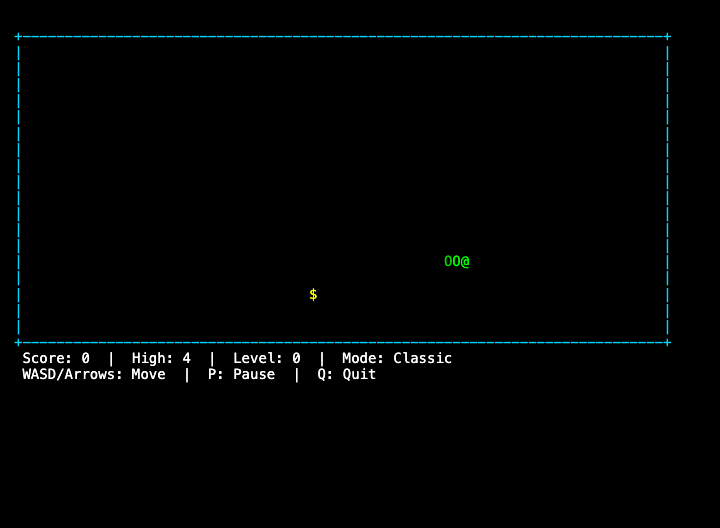
\includegraphics[width=0.46\columnwidth]{figures/gameplay_classic.png}\hfill
    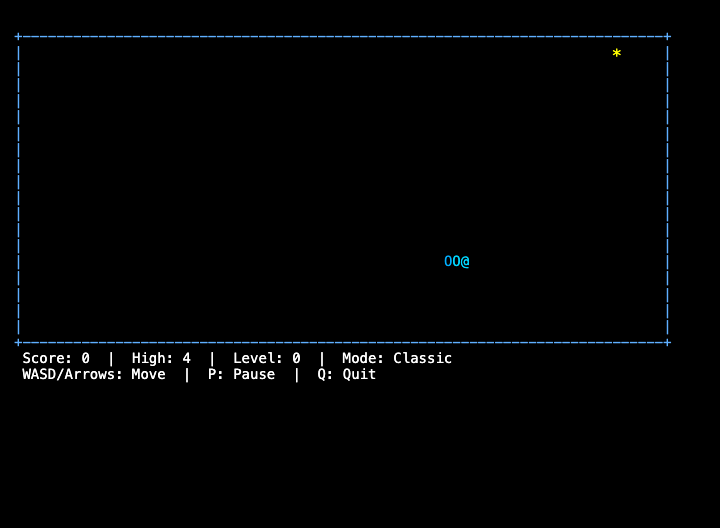
\includegraphics[width=0.46\columnwidth]{figures/gameplay_ice.png}\\[3pt]
    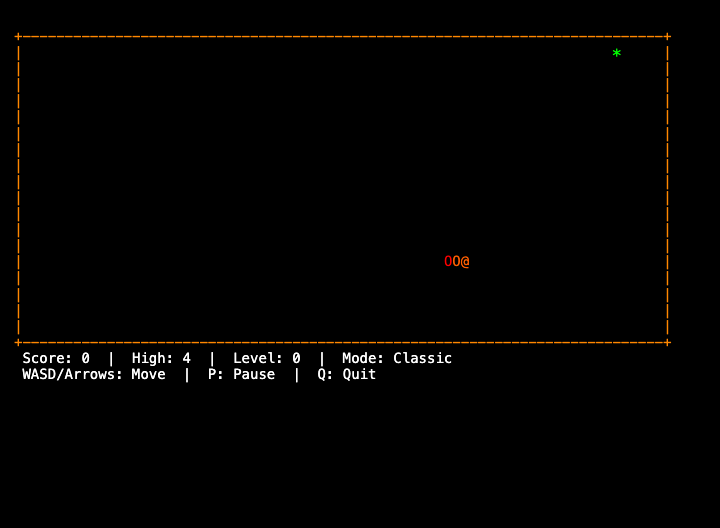
\includegraphics[width=0.46\columnwidth]{figures/gameplay_lava.png}\hfill
    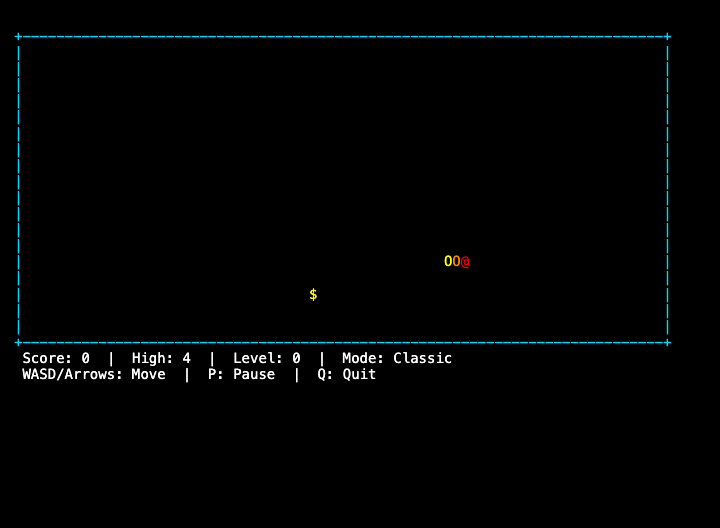
\includegraphics[width=0.46\columnwidth]{figures/gameplay_rainbow.png}
    \caption{All four themes. Top row: Classic (green), Ice (blue). Bottom row: Lava (red/orange), Rainbow (cycling). The HUD and border colours adapt with each theme.}
    \label{fig:themes}
\end{figure}

\subsection{Two Game Modes}
The board exposes two collision policies, selected on the title screen:
\begin{itemize}
    \item \textbf{Classic mode} -- the wall is lethal; running into the border kills the snake.
    \item \textbf{Wrap-Around mode} -- the board behaves as a torus; coordinates leaving any edge re-enter on the opposite edge via the branch-free \texttt{my\_mod} expression of Listing~\ref{lst:wrap} (see Fig.~\ref{fig:wrap}).
\end{itemize}

\begin{figure}[H]
    \centering
    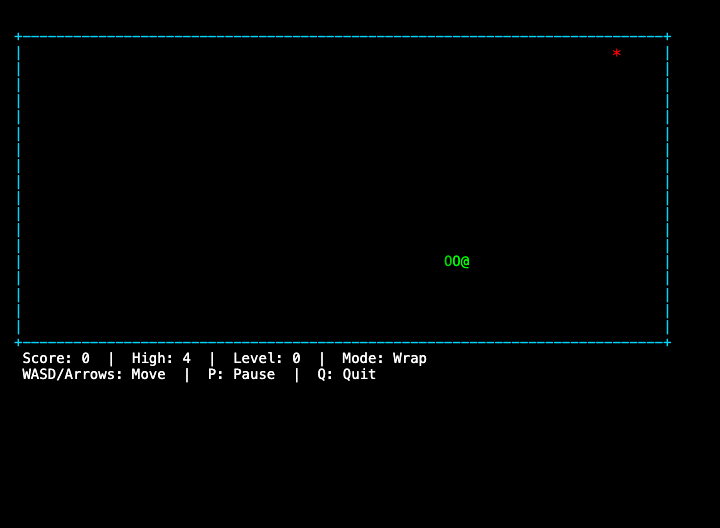
\includegraphics[width=0.92\columnwidth]{figures/gameplay_wrap.png}
    \caption{Wrap-Around mode. The HUD reads \texttt{Mode: Wrap}; the snake can leave any wall and re-emerge on the opposite side.}
    \label{fig:wrap}
\end{figure}

%==============================================================================
\section{Phase~2 Developmental Features}
\label{sec:phase2}

In addition to the Phase~1 build documented above (branch \texttt{main} / \texttt{feature/endsem-submission}), a Phase~2 branch (\texttt{ravi/phase2}) extends the core game with several advanced mechanics. These extensions inherit the same custom libraries, allocator, and rendering pipeline; they exercise the same OS sub-systems but at a higher level of game complexity.

\subsection{Multi-Food Spawning}
The food module is generalised from a single \texttt{Food*} to a \texttt{Foods} container holding up to several pieces simultaneously. Each piece carries its own type and despawn timer; the collision and respawn logic of Section~\ref{sec:methodology} is iterated across the array. This raises the average tick speed without raising the difficulty floor, because the player has more targets to chase.

\subsection{Ghost Snake (Autonomous AI Body)}
A second snake (\texttt{Snake *ghost}) moves on the same board under autonomous control. Each tick \texttt{ghost\_step()} chooses a direction with the same custom PRNG used for food and obstacle placement (Listing~\ref{lst:prng}) and moves the ghost; its body is rendered in a distinct colour (Fig.~\ref{fig:phase2gameplay}, purple \texttt{oog}) and acts as a moving obstacle. The collision pipeline is extended so that landing on any ghost segment is lethal in Classic mode.

\subsection{Power-Up Zones}
Discrete power-up zones are spawned with a cooldown and a fixed lifetime. Two types are implemented:
\begin{itemize}
    \item \texttt{POW\_BOOST} -- temporarily speeds the snake for 25 ticks.
    \item \texttt{POW\_SLOW} -- temporarily slows the snake for 25 ticks.
\end{itemize}
Zones glow with an animated colour cycle driven by a per-zone \texttt{glow\_phase} counter, and they participate in obstacle/food/snake placement-safety checks via \texttt{powerups\_find\_at()}.

\subsection{Shrinking Board (Inset)}
The play area shrinks over time via a configurable inset. The board module exposes \texttt{board\_in\_play\_area()} which all collision and spawn checks consult, so the shrink mechanism is enforced without modifying every caller. As the inset grows, food and power-ups outside the new play area are dropped through \texttt{powerups\_drop\_invalid()}.

\subsection{Replay (Best-Run Ghost)}
A persistent replay system records the head position of every tick into a \texttt{Replay} struct (capacity 6{,}000 frames; each frame is a pair of \texttt{short} coordinates = 4~bytes, so $\approx$24\,KB total). When a run scores higher than the saved best, the trajectory is written to disk; subsequent runs load the best replay and render it as a translucent ``ghost'' that the player can race against. This pattern is the same one used by deterministic-replay debuggers in real OS schedulers.

\subsection{Dynamic Terminal Resize Handling}
Phase~2 honours \texttt{SIGWINCH}-style window changes: \texttt{wait\_for\_valid\_terminal()} polls the terminal dimensions and pauses the game until the window meets the minimum size, after which \texttt{apply\_terminal\_resize()} re-clamps board geometry, drops out-of-bounds entities, and triggers a full redraw via \texttt{redraw\_full\_game()}. Figure~\ref{fig:phase2themes} shows the Phase~2 build running across all four themes and both collision modes; every screenshot was generated by the same scripted pipeline that produced the Phase~1 figures.

\begin{figure}[H]
    \centering
    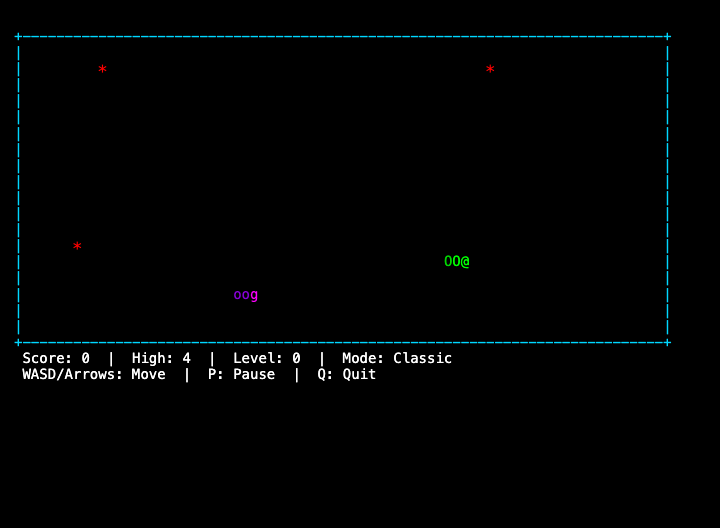
\includegraphics[width=0.92\columnwidth]{figures/phase2_gameplay_classic.png}
    \caption{Phase~2 build in action. Three red \texttt{*} food pieces are spawned simultaneously (multi-food); the purple \texttt{oog} body in the lower-middle is the autonomous ghost snake; the player snake \texttt{00@} is in green at the right.}
    \label{fig:phase2gameplay}
\end{figure}

\begin{figure}[H]
    \centering
    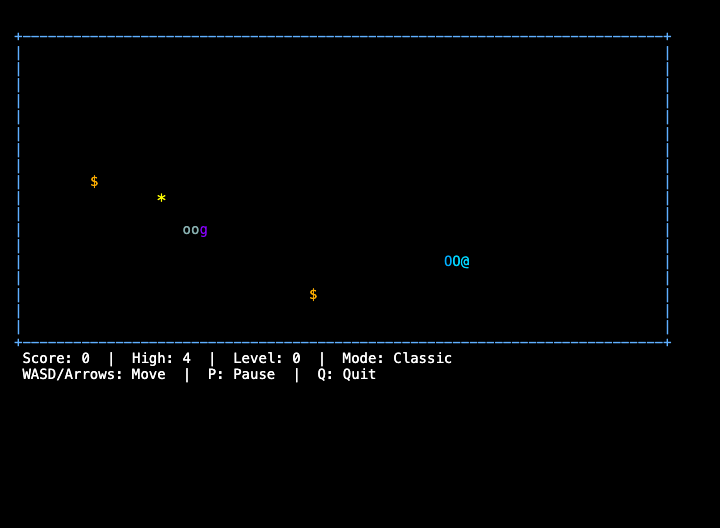
\includegraphics[width=0.46\columnwidth]{figures/phase2_gameplay_ice.png}\hfill
    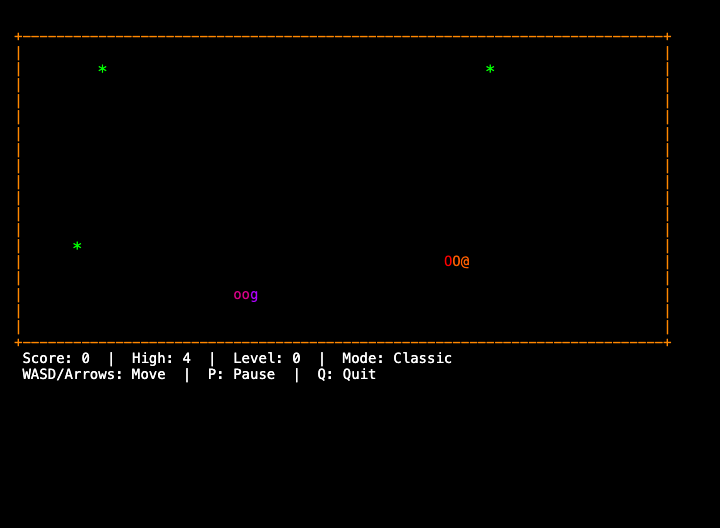
\includegraphics[width=0.46\columnwidth]{figures/phase2_gameplay_lava.png}\\[3pt]
    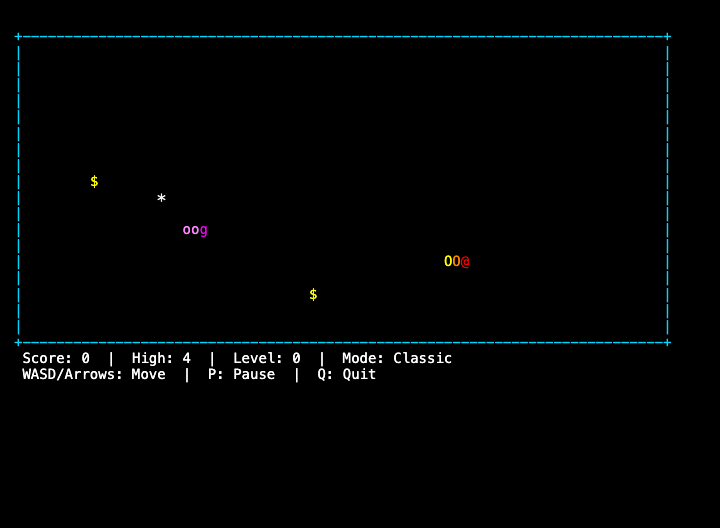
\includegraphics[width=0.46\columnwidth]{figures/phase2_gameplay_rainbow.png}\hfill
    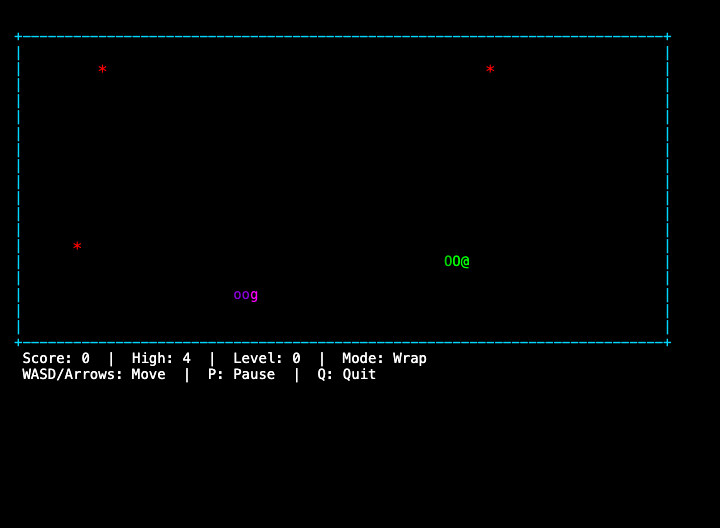
\includegraphics[width=0.46\columnwidth]{figures/phase2_gameplay_wrap.png}
    \caption{Phase~2 across themes and modes. Top row: Ice and Lava themes with multi-food + ghost snake. Bottom row: Rainbow theme; Wrap-Around mode with the toroidal collision policy of Listing~\ref{lst:wrap}.}
    \label{fig:phase2themes}
\end{figure}

%==============================================================================
\section{Results and Testing}
\label{sec:results}

\subsection{Build}
The project builds cleanly under \texttt{gcc} with \texttt{-Wall -Wextra -Werror} on macOS Darwin~25.4.0 and Linux. A \texttt{Makefile} provides six phony targets: \texttt{all}, \texttt{run}, \texttt{test}, \texttt{clean}, \texttt{screenshots} (drives the binary in a real Terminal.app window via \texttt{osascript}+\texttt{screencapture}), and \texttt{screenshots-headless} (drives the binary inside a \texttt{tmux} pseudo-terminal and converts the captured ANSI to PNG via \texttt{aha} and headless Chromium). Total binary size is approximately 91\,KB.

\subsection{Reproducible Screenshot Pipeline}
The \texttt{scripts/capture\_screenshots.sh} driver scripts a complete play-through: it launches the binary inside a 80$\times$24 \texttt{tmux} session, uses \texttt{tmux send-keys} to inject mode/theme selections and arrow-key inputs at a fixed cadence, snapshots the pane after each milestone with \texttt{tmux capture-pane -e}, converts the captured ANSI sequence to a self-contained HTML document via \texttt{aha}, and finally renders the HTML to PNG using a headless Chromium browser. A companion script \texttt{capture\_phase2.sh} adds a \texttt{git worktree} on the \texttt{ravi/phase2} branch, builds the Phase~2 binary, and reuses the same driver to produce phase-2 screenshots without disturbing the \texttt{main} checkout. This pipeline guarantees that every figure in this report can be regenerated identically by typing \texttt{make screenshots-headless}.

\subsection{Unit Tests}
Three test suites exercise the system libraries:
\begin{itemize}
    \item \textbf{math} -- 32 cases covering multiply, divide, mod, abs, min, max, clamp, and PRNG period.
    \item \textbf{string} -- 19 cases covering \texttt{strlen}, \texttt{strcpy}, \texttt{strcmp}, \texttt{strcat}, and integer/string conversions.
    \item \textbf{memory} -- 14 cases covering allocation, deallocation, coalescing, fragmentation, and out-of-memory behaviour.
\end{itemize}
All 65 tests pass under \texttt{make test}.

\subsection{Functional Demonstration}
Figures~\ref{fig:title}--\ref{fig:gameover} show representative screenshots from a play session.

\begin{figure}[H]
    \centering
    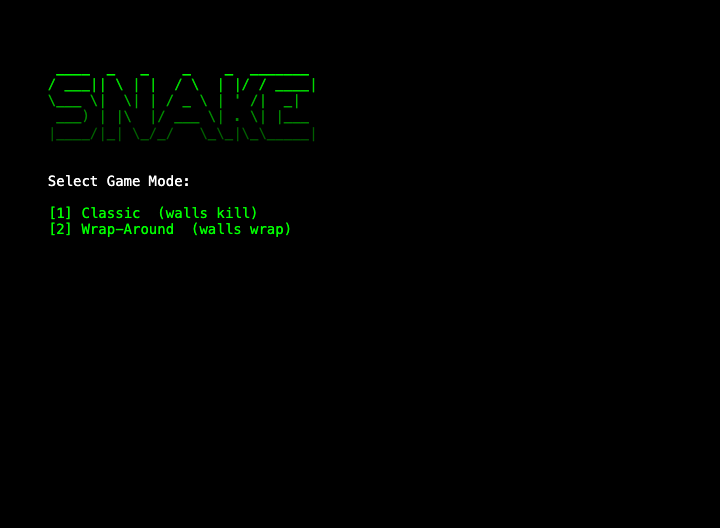
\includegraphics[width=0.92\columnwidth]{figures/title.png}
    \caption{Title screen with the gradient ASCII ``SNAKE'' banner and game-mode selection (Classic / Wrap-Around).}
    \label{fig:title}
\end{figure}

\begin{figure}[H]
    \centering
    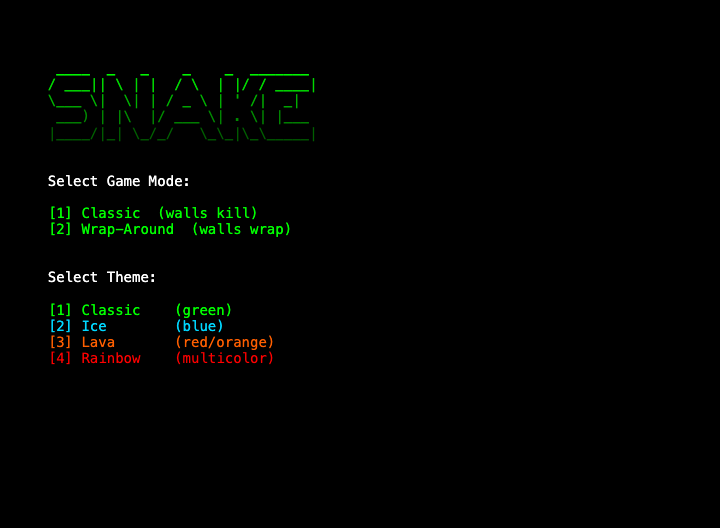
\includegraphics[width=0.92\columnwidth]{figures/theme.png}
    \caption{Theme-selection screen offering Classic, Ice, Lava, and Rainbow palettes; each entry is rendered in its own colour as a live preview.}
    \label{fig:theme}
\end{figure}

\begin{figure}[H]
    \centering
    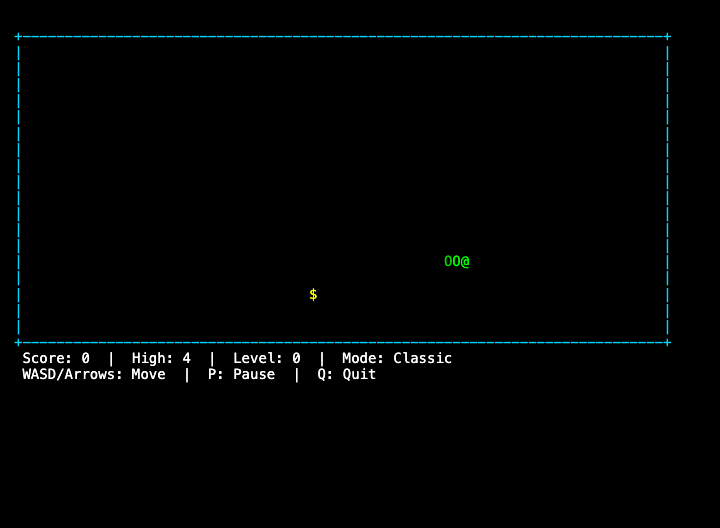
\includegraphics[width=0.92\columnwidth]{figures/gameplay.png}
    \caption{In-game state in Classic mode with the Classic theme: green gradient snake (\texttt{00@}), red food (\texttt{*}), cyan dashed border, and the two-line HUD showing score, high-score, level, mode, and key bindings.}
    \label{fig:gameplay}
\end{figure}

\begin{figure}[H]
    \centering
    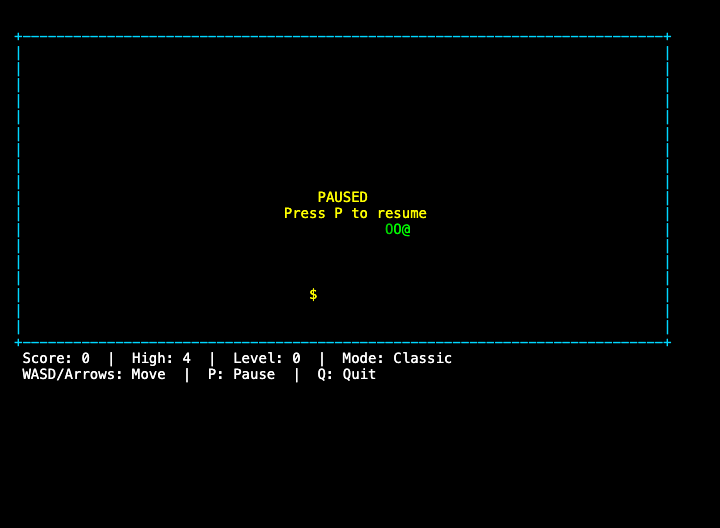
\includegraphics[width=0.92\columnwidth]{figures/pause.png}
    \caption{Pause overlay (after pressing \texttt{P}). The game state is preserved exactly; the loop only polls the keyboard.}
    \label{fig:pause}
\end{figure}

\begin{figure}[H]
    \centering
    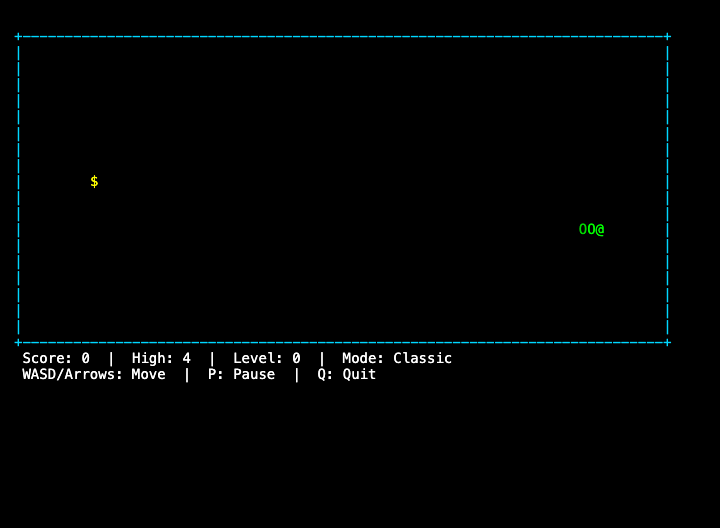
\includegraphics[width=0.92\columnwidth]{figures/gameover.png}
    \caption{Game-over screen showing the death animation, final and high score, and the lifetime statistics panel (games played, total food, longest snake, best level) -- all values are persisted to \texttt{data/stats.dat}.}
    \label{fig:gameover}
\end{figure}

\subsection{Version Control}
The project is hosted publicly on GitHub at \url{https://github.com/HackHeroic/Snake_game_os}. The repository organises work across multiple branches:
\begin{itemize}
    \item \texttt{main} / \texttt{feature/endsem-submission} -- the stable Phase~1 submission documented in Sections~\ref{sec:methodology}--\ref{sec:impl}.
    \item \texttt{ravi/phase2} -- the Phase~2 extensions (multi-food, ghost snake, power-ups, shrinking board, replay) documented in Section~\ref{sec:phase2}.
    \item \texttt{phase2/features} -- exploratory work on individual phase~2 features.
\end{itemize}
Significant milestones include:
\begin{itemize}
    \item \texttt{feat: snake game core} -- baseline gameplay, custom libraries.
    \item \texttt{feat: special food types} -- bonus and slow food.
    \item \texttt{feat: obstacles, themes, stats} -- level-up obstacles, four colour themes, persisted lifetime statistics.
    \item \texttt{feat: multi food logic} -- generalised \texttt{Food*} to \texttt{Foods} container.
    \item \texttt{feat: ghost snake} -- autonomous AI body sharing the board.
    \item \texttt{feat: phase~2 features} -- power-up zones, shrinking board, replay ghost.
    \item \texttt{fix: dynamic terminal resize} -- \texttt{SIGWINCH}-aware redraw and clamp.
    \item \texttt{fix: resize ghosting} -- residual cells purged on inset shrink.
    \item \texttt{fix: obstacles\_init before food\_spawn} -- avoids reading uninitialised memory.
    \item \texttt{docs: implementation document, viva docs, README updates}.
\end{itemize}
A linear, well-described commit history serves as both an evaluation artefact and a reproducibility guarantee.

%==============================================================================
\section{Future Scope}
\label{sec:future}

The current system covers all five OS sub-systems but several interesting extensions remain.

\paragraph{(a) Multi-threaded Rendering and Input}
Splitting the game loop into a renderer thread and an input thread would decouple frame timing from input latency. Synchronisation would require introducing a small POSIX-thread mutex layer, providing a teaching opportunity for race conditions and deadlock.

\paragraph{(b) Free-Block Lists for the Allocator}
The current first-fit traversal is $O(n)$ in the number of blocks. Maintaining an explicit free-list (and, optionally, segregated free-lists by size class) would reduce average allocation time at the cost of additional bookkeeping.

\paragraph{(c) Networked Multiplayer}
A simple TCP server in front of two game instances would demonstrate I/O multiplexing via \texttt{select} or \texttt{epoll}. The existing strict separation of \texttt{game/} from \texttt{ui/} makes this conceptually straightforward.

\paragraph{(d) Crash-Safe File System}
Replacing the current rewrite-in-place save with a copy-on-write rename pattern (write to \texttt{stats.dat.tmp}, \texttt{rename} into place) would survive a crash mid-write, mirroring the journaling approach used by ext4 and APFS~\cite{silberschatz2018}.

\paragraph{(e) Network-Synchronised Ghost Snakes}
Phase~2 already implements a local ghost snake (Section~\ref{sec:phase2}); a natural next step is to share ghost trajectories between users over a small UDP protocol so that two players can race each other's best runs asynchronously.

\paragraph{(f) Sandboxed Resource Limits}
Setting \texttt{rlimit} bounds on CPU and memory at start-up would demonstrate kernel-enforced security, complementing the application-level invariants already in place.

\paragraph{(g) Replay-File Format Stability}
The Phase~2 replay system writes a fixed-size binary record. A versioned, length-prefixed format (with a magic number and forward-compatible reserved fields) would let future builds read older replays, much as ext4 reads ext2 superblocks.

\paragraph{(h) Audio via Coreaudio / ALSA}
A single-channel beep on food intake and game-over would round out the I/O subsystem and demonstrate device management beyond the terminal.

%==============================================================================
\section{Conclusion}
\label{sec:conclusion}

We presented \textit{Snake Game OS}, a real-time terminal Snake game in which all five canonical operating-systems sub-systems---memory, processes, files, I/O, and security---are implemented from first principles in approximately 1{,}500 lines of C. The design choices are deliberate and defensible: a first-fit allocator with coalescing matches the small, homogeneous workload; a deterministic game-loop scheduler with a three-state FSM models a cooperative process; a delta-render strategy over ANSI escape codes eliminates flicker; flat ASCII files persist user data; and a coordinated halt protocol guarantees terminal restoration on every exit path. A separate Phase~2 branch lifts the engine to a higher complexity tier with multi-food, an autonomous ghost AI, power-up zones, a shrinking board, persistent best-run replay, and \texttt{SIGWINCH}-aware resize handling -- all built atop the same five sub-systems without bypassing the custom allocator or the strict header allow-list. The 65 unit tests, the strict \texttt{-Werror} build, the scripted screenshot pipeline, and the public GitHub history together form an evaluation surface that is reproducible, inspectable, and pedagogically transparent.

\FloatBarrier
%==============================================================================
\begin{thebibliography}{9}

\bibitem{silberschatz2018}
A.~Silberschatz, P.~B.~Galvin, and G.~Gagne, \emph{Operating System Concepts}, 10th~ed.\ Hoboken, NJ: Wiley, 2018.

\bibitem{tanenbaum2014}
A.~S.~Tanenbaum and H.~Bos, \emph{Modern Operating Systems}, 4th~ed.\ Upper Saddle River, NJ: Pearson, 2014.

\bibitem{knuth1997}
D.~E.~Knuth, \emph{The Art of Computer Programming, Volume~1: Fundamental Algorithms}, 3rd~ed.\ Reading, MA: Addison-Wesley, 1997.

\bibitem{wilson1995}
P.~R.~Wilson, M.~S.~Johnstone, M.~Neely, and D.~Boles, ``Dynamic storage allocation: A survey and critical review,'' in \emph{Proc.\ Int.\ Workshop Memory Mgmt.}, Sept.~1995, pp.~1--116.

\bibitem{park1988}
S.~K.~Park and K.~W.~Miller, ``Random number generators: Good ones are hard to find,'' \emph{Commun.\ ACM}, vol.~31, no.~10, pp.~1192--1201, Oct.~1988.

\bibitem{schrage1979}
L.~Schrage, ``A more portable Fortran random number generator,'' \emph{ACM Trans.\ Math.\ Softw.}, vol.~5, no.~2, pp.~132--138, June~1979.

\bibitem{ncurses}
T.~E.~Dickey, \emph{NCURSES---New Curses}, GNU project documentation, 2024. [Online]. Available: \url{https://invisible-island.net/ncurses/}

\bibitem{ansi}
\emph{Information technology---Control functions for coded character sets}, ECMA Standard 48, 5th~ed., June~1991.

\bibitem{posix}
IEEE Std 1003.1-2017 (Revision of IEEE Std 1003.1-2008), \emph{IEEE Standard for Information Technology---Portable Operating System Interface (POSIX)}, IEEE, 2018.

\end{thebibliography}

\end{document}
